\begin{center}
	\begin{circuitfig}[H]
		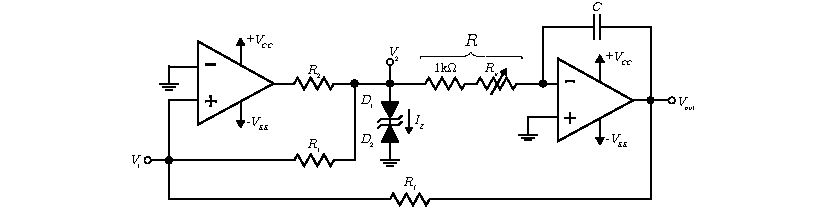
\includegraphics[width=\textwidth]{circuits/micro3_lab1.pdf}
		\caption{Γεννήτρια τριγωνικής παλμοσειράς.}
		\label{circ:1_schematic}
	\end{circuitfig}
\end{center}
\vspace*{-1cm}

Στην πρώτη άσκηση μελετάται το κύκλωμα \ref{circ:1_schematic} το οποίο αποτελείται από δύο τελεστικούς ενισχυτές 741. Για την τροφοδοσία των τελεστικών ενισχυτών είναι $V_{CC}=15\unit{\volt}$ και $V_{EE}=15\unit{\volt}$. Οι δύο δίοδοι Zener (1N750) έχουν τάση Zener $V_Z=7.5\unit{\volt}$ και τάση στην ορθή πόλωση $V_D=0.7\unit{\volt}$.\par
Για τους ωμικούς αντιστάτες είναι $R_2=4.7\unit{\kilo\ohm}$ και $R=40\unit{\kilo\ohm}$. Για τις υπόλοιπες αντιστάσεις, $R_1,R_f$, και τον πυκνωτή, $C$, βάσει των οδηγιών προκύπτει $R_1=50\unit{\kilo\ohm}$, $R_f=35\unit{\kilo\ohm}$ και $C=4\unit{\nano\farad}$. Ωστόσο, επιλέχθηκαν οι πλησιέστερες τιμές που εμφανίζονται στα τυποποιημένα εξαρτήματα. Τελικα, το κύκλωμα υλοποιήθηκε με $R_1=47\unit{\kilo\ohm}$, $R_f=33\unit{\kilo\ohm}$ και $C=4.7\unit{\nano\farad}$.\par

\section{Θεωρητική μελέτη \& προσομοίωση}

	\subsection{Περιγραφή της λειτουργίας του κυκλώματος}
		\vspace{10pt}
\begin{wrapfigure}{R}{0.25\textwidth}
	\begin{minipage}{0.25\textwidth}
		\pgfplotsset{grid style={dotted,lightgray}}
		\begin{tikzpicture}[>=latex]
			\begin{axis}[
				width=5.2cm,
				height=6cm,
				grid,
				axis x line=middle,
				axis y line=middle,
				% ==================
				xmin=-3,
				xmax=3,
				xtick={-1.5,0,1.5},
				xticklabels={$V_{LTP}$,$V_{ref}$,$V_{UTP}$},
				x tick label style={rotate=60,anchor=east},
				xlabel={$V_1$},
				ylabel style={right},
				% ==================
				ymin=-10,
				ymax=10,
				ytick={-8,8},
				yticklabels={},
				ylabel={$V_2$},
				ylabel style={above}]
				\addplot[thick, const plot, color=DodgerBlue3]
				coordinates	{(-1.5,-8) (-1.5,8) (5,8)};
				\addplot[thick, const plot, color=DeepPink3]
				coordinates	{(-5,-8) (1.5,-8) (1.5,8)};
				% ==================
				\addplot[->,mark=none, color=DodgerBlue3] coordinates {(-1.5,-3) (-1.5,-3.5)};
				\addplot[->,mark=none, color=DodgerBlue3] coordinates {(-1.5,+3.5) (-1.5,3)};
				\addplot[->,mark=none, color=DodgerBlue3] coordinates {(1,8) (0.5,8)};
				% ==================
				\addplot[->,mark=none, color=DeepPink3] coordinates {(1.5,3) (1.5,3.5)};
				\addplot[->,mark=none, color=DeepPink3] coordinates {(1.5,-3.5) (1.5,-3)};
				\addplot[->,mark=none, color=DeepPink3] coordinates {(-1,-8) (-0.5,-8)};
				% ==================
				\node[anchor=east] at (axis cs:-1.5, 8) {$L_{+}$};
				\node[anchor=west] at (axis cs:1.5, -8) {$L_{-}$};
			\end{axis}
		\end{tikzpicture}
	\end{minipage}
	\caption{Χαρακτηριστική ενός Schmitt trigger με στάθμη αναφοράς $0\unit{\volt}$.}
\end{wrapfigure}


Το κύκλωμα \ref{circ:1_schematic} απαρτίζεται από ένα δισταθές κύκλωμα (αριστερά τελεστικός ενισχυτής) σε ρόλο συγκριτή με θετική ανάδραση (noninverting Schmitt trigger) και έναν ολοκληρωτή (δεξιά τελεστικός ενισχυτής). Επιπλέον, στην έξοδο του συγκριτή υπάρχει waveform clipping κύκλωμα το οποίο υλοποιείται με δύο διόδους Zener συνδεδεμένες \textsl{back-to-back}.\par

\subsubsection{Noniverting Schmitt trigger}
	Έστω $L_{+}$ η θετική στάθμη (ή θετική τάση κορεσμού) του δισταθούς κυκλώματος και $L_{-}$ η αρνητική στάθμη του. Εάν η έξοδος του συγρκιτή βρίσκεται στη θετική στάθμη, $L_{+}$, τότε προκειμένου να αλλάξει κατάσταση και να μεταβεί στην αρνητική στάθμη, $L_{-}$ θα πρέπει η τάση στην μη αναστρέφουσα είσοδο του τελεστικού ενισχυτή να γίνει οριακά μικρότερη του lower trip point $V_{LTP}(L_+)$.\cite{malvino}\cite{sedra} Τότε, η έξοδος του συγκριτή περνάει και παραμένει στην αρνητική στάθμη $L_{-}$ έως ότου η τάση στην μη αναστρέφουσα είσοδο του τελεστικού ενισχυτή να γίνει οριακά μεγαλύτερη του upper trip point $V_{UTP}(L_-)$.\cite{malvino}\cite{sedra} Τέλος, αξίζει να σημειωθεί πως γειώνοντας την αναστρέφουσα είσοδο του τελεστικού ενισχυτή, η στάθμη αναφοράς είναι τα $0\unit{\volt}$. Επομένως, είναι $V_{LTP}<0$ και $V_{UTP}>0$.\par
	\vspace*{10pt}
	Στην έξοδο του συγκριτή, $v_2$, εμφανίζεται ένας τετραγωνικός παλμός με μέγιστη τιμή $V_{\Pi,\max}\simeq L_{+}$ και ελάχιστη τιμή $V_{\Pi,\min}\simeq L_{-}$\cite{sedra}, εάν $L_{+},|L_{-}|\leqslant|V_D+V_Z|$. Δηλαδή, η μέγιστη, κατά απόλυτη τιμή, έξοδος του συγκριτή είναι $|V_D+V_Z|$. Ο περιορισμός αυτός επιβάλλεται απο τις διόδους Zener. Όταν η έξοδος του συγκριτή βρίσκεται στη θετική στάθμη, η δίοδος $D_1$ θα είναι πολωμένη ορθά διατηρώντας σταθερή διαφορά δυναμικού μεταξύ των άκρων της $V_D=0.7V$ και η $D_2$ θα βρίσκεται στην περιοχή Zener. Επομένως, η κυματομορφή θα έχει άνω όριο $V_D+V_Z$. Ομοίως, εάν η έξοδος του συγκριτή βρίσκεται στην αρνητική στάθμη, η $D_1$ θα είναι αναστροφα πολωμένη και θα λειτουργεί στην περιοχή Zener και η $D_2$ θα είναι ορθά πολωμένη. Συνεπώς, η κυματομορφή $v_2$ θα έχει κάτω όριο $-\(V_D+V_Z\)$.\par

\subsubsection{Ολοκληρωτής}
	Η έξοδος του συγκριτή συνδέεται μέσω ωμικού αντιστάτη $R$ στην αναστρέφουσα είσοδο του τελεστικού ενισχυτή του ολοκληρωτή. Θεωρώντας πως οι τελεστικοί ενισχυτές είναι ιδανικοί, το ρεύμα εισόδου στον αναστρέφων ακροδέκτη του τελεστικού ενισχυτή είναι μηδέν (καθώς η αντίσταση εισόδου είναι άπειρη). Εξαιτίας της εικονικής γείωσης του αναστρέφοντος ακροδέκτη, το ρεύμα που διαρρέει την αντίσταση $R$ είναι $\displaystyle{i=\sfrac{v_2}{R}}$ και διαρρέει και τον πυκνωτή χωρητικότητας $C$. Η έξοδος $v_{\mathrm{out}}$ δίνεται από τη σχέση
	\begin{equation}
		v_{\mathrm{out}}(t)=v_{\mathrm{out}}(0)-\frac{1}{C}\int{i(t)\dd{t}}\Longleftrightarrow v_{\mathrm{out}}(t)=v_{\mathrm{out}}(0)-\frac{1}{R\cdot C}\int{v_2(t)\dd{t}}
		\label{eq:1_vout_integrator}
	\end{equation}


\subsubsection{Συνολική λειτουργία}
	Έστω πως η έξοδος του συγκριτή ξεκινάει από την θετική στάθμη. Όσο η τάση $v_{\mathrm{out}}$ είναι μεγαλύτερη της $V_{LTP}$ η $v_2$ παραμένει σταθερή. Συνεπώς και το ρεύμα $i$ είναι σταθερό ως προς τον χρόνο στο διάστημα αυτό και ίσο με $i^{(+)}=\sfrac{v_2^{(+)}}{R}$. Τότε, η σχέση \eqref{eq:1_vout_integrator} γίνεται
	\begin{equation*}
		v_{\mathrm{out}}=v_{\mathrm{out}}(0)-\frac{v_2^{(+)}}{R\cdot C}t.
	\end{equation*}
	Δηλαδή, η έξοδος μειώνεται γραμμικά ως προς τον χρόνο με κλίση $\displaystyle{-\sfrac{v_2^{(+)}}{\(R\cdot C\)}}$ έως ότου η $v_{\mathrm{out}}$ να γίνει οριακά μικρότερη της $V_{LTP}$. Τότε, η έξοδος του συγκριτή μεταβάλλεται στην αρνητική στάθμη. Επομένως, το ρεύμα που διαρρέει τον αντιστάτη $R$ και τον πυκνωτή $C$ είναι $i^{(-)}=\sfrac{v_2^{(-)}}{R}$ και είναι αντίθετης φοράς του $i^{(+)}$. Βάσει της σχέσης \eqref{eq:1_vout_integrator} η έξοδος του ολοκληρωτή είναι
	\begin{equation*}
		v_{\mathrm{out}}=v_{\mathrm{out}}(0)-\frac{-v_2^{(-)}}{R\cdot C}t.
	\end{equation*}
	Είναι προφανές από την παραπάνω σχέση πως η έξοδος $v_{\mathrm{out}}$ θα αυξάνει γραμμικά ως προς τον χρόνο με κλίση $\displaystyle{\sfrac{v_2^{(-)}}{\(R\cdot C\)}}$ έως ότου η $v_{\mathrm{out}}$ να γίνει οριακά μεγαλύτερη της $V_{UTP}$.\par

	Συνοψίζοντας τα παραπάνω, για την έξοδο της γεννήτριας θα ισχύει
	\begin{equation*}
		\frac{v_1-v_2}{R_1}=\frac{v_{\mathrm{out}}-v_1}{R_f}
	\end{equation*}
	ή
	\begin{equation}
		\label{eq:ask1_vout}
		v_{\mathrm{out}}(t)=v_1(t)+R_f\cdot\frac{v_1(t)-v_2(t)}{R_1}.
	\end{equation}

	Από την σχέση \eqref{eq:ask1_vout} φαίνεται πως η εναλλαγή των καταστάσεων του δισταθούς κυκλώματος και τα ολικά ακρότατα του τριγωνικού παλμού της εξόδου λαμβάνονται τις στιγμές $t=\sfrac{kT}{2},k\in\mathbb{N}$ ($T$ η περίοδος του σήματος) όπου $v_1=0\unit{\volt}$.

	Θέτοντας $\displaystyle{v_{\mathrm{out}}\(\sfrac{kT}{2}\)=v_2\cdot\(\sfrac{R_f}{R_1}\),k\in\mathbb{N}}$ η περίοδος του τριγωνικού παλμού, υπό την προϋπόθεση πως τα $L_{+}$ και $-L_{-}$ είναι ίσα\cite{sedra}, θα είναι\cite{malvino}
	\begin{equation}
		\label{eq:ask1_period}
		T=2\cdot R\cdot C\cdot 2\frac{R_f}{R_1}=4\frac{R\cdot C\cdot R_f}{R_1}
	\end{equation}
	ή εναλλακτικα, η έκφραση για τη συχνότητα του σήματος θα είναι
	\begin{equation}
		\label{eq:ask1_freq}
		f=\frac{R_1}{4\cdot R\cdot C\cdot R_f}.
	\end{equation}

	% \subsection{Προσομοίωση με PSpice}

	% \subsection{Μέγιστη συχνότητα λειτουργίας}

	% \subsection{Ρύθμιση του πλάτους τους σήματος}

\section{Εργαστηριακή εφαρμογή}

	\subsection{Λήψη κυματομορφών $V_1$, $V_2$ και $V_{\mathrm{out}}$}
		Οι κυματομορφές $V_{\mathrm{out}}, V_1$ και $V_2$ του κυκλώματος \ref{circ:1_schematic} σε διάστημα  $1.184\unit{\milli\second}$ για $R_1=47\unit{\kilo\ohm}$, $R_2=4.7\unit{\kilo\ohm}$, $R_v=39.4\unit{\kilo\ohm}\rightarrow R=40.4\unit{\kilo\ohm}$, $R_f=33\unit{\kilo\ohm}$ και $C=4.7\unit{\nano\farad}$ δίδονται στο διάγραμμα \ref{plot:1_lab_voltages}.

		\begin{chart}[H]
			\begin{center}
				\pgfplotsset{grid style={dotted,lightgray}}
\begin{tikzpicture}
	\begin{axis}[
	grid=both,
	minor tick num=1,
	xticklabels={},
	ymin=-15,
	ymax=15,
	xtick={0,200,400,600,800,1000,1200},
	xticklabels={0,200,400,600,800,1000,1200},
	ytick={-10,-5,0,5,10},
	xlabel={Time $\(\unit{\micro\second}\)$},
	ylabel={Voltage $\(\unit{\volt}\)$}]
	\addplot+[thick,mark=none,const plot,color=DodgerBlue3]
		coordinates	{(0,0) (0,9) (0.5*592,-8) (592,9) (1.5*592,-8) (2*592,0)};
	\addplot+[thick,mark=none,domain=0:2*592,color=DeepPink3]
		coordinates {(0,6.8) (0.5*592,-7) (592,6.8) (1.5*592,-7) (2*592,6.8)};
	\addplot+[dashed,thick,mark=none,domain=0:2*592,color=black]
		coordinates {(0,0) (0,6.8) (0.5*592,0) (0.5*592,-7) (592,0) (592,6.8) (1.5*592,0) (1.5*592,-7) (2*592,0)};
	\legend{$V_2$,$V_{\mathrm{out}}$,$V_1$}
	\end{axis}
\end{tikzpicture}
				\caption{Οι τάσεις $V_1, V_2$ και $V_{\mathrm{out}}$ όπως μετρήθηκαν χρήσει του παλμογράφου στο εργαστήριο.}
				\label{plot:1_lab_voltages}
			\end{center}
		\end{chart}